\documentclass[12pt]{article} % use larger type; default would be 10pt
\usepackage[czech]{babel}
\usepackage[utf8]{inputenc} % set input encoding (not needed with XeLaTeX)

%%% PAGE DIMENSIONS
\usepackage{geometry} % to change the page dimensions
% \usepackage[left=2cm,right=2cm,top=2cm,bottom=2cm]{geometry}
\geometry{a4paper}
% \geometry{margin=2in} % for example, change the margins to 2 inches all round
% \geometry{landscape} % set up the page for landscape

\usepackage{graphicx} % support the \includegraphics command and options
\usepackage{wrapfig} % support the wrapfigure section

\usepackage{tikz} % graphs
\usepackage{pgfplots}

\usepackage{hyperref} % links in \tableofcontents
\hypersetup{
	colorlinks,
	citecolor=black,
	filecolor=black,
	linkcolor=black,
	urlcolor=black
}

% \usepackage[parfill]{parskip} % Activate to begin paragraphs with an empty line rather than an indent

%%% PACKAGES
\usepackage{booktabs} % for much better looking tables
\usepackage{array} % for better arrays (eg matrices) in maths
% \usepackage{paralist} % very flexible & customisable lists (eg. enumerate/itemize, etc.)
\usepackage{verbatim} % adds environment for commenting out blocks of text & for better verbatim
\usepackage{subfig} % make it possible to include more than one captioned figure/table in a single float
% These packages are all incorporated in the memoir class to one degree or another...
\usepackage{float}

%%% HEADERS & FOOTERS
\usepackage{fancyhdr} % This should be set AFTER setting up the page geometry
\pagestyle{fancy} % options: empty , plain , fancy
\renewcommand{\headrulewidth}{0pt} % customise the layout...
\lhead{}\chead{}\rhead{}
\lfoot{}\cfoot{\thepage}\rfoot{}

%%% SECTION TITLE APPEARANCE
\usepackage{sectsty}
\allsectionsfont{\sffamily\mdseries\upshape} % (See the fntguide.pdf for font help)
% (This matches ConTeXt defaults)

%%% ToC (table of contents) APPEARANCE
\usepackage[nottoc,notlof,notlot]{tocbibind} % Put the bibliography in the ToC
\usepackage[titles,subfigure]{tocloft} % Alter the style of the Table of Contents
\renewcommand{\cftsecfont}{\rmfamily\mdseries\upshape}
\renewcommand{\cftsecpagefont}{\rmfamily\mdseries\upshape} % No bold!
\newcommand{\bigsize}{\fontsize{35pt}{20pt}\selectfont}

%%% END Article customizations

\begin{document}
\begin{titlepage}
	
\includegraphics[scale=0.7]{logo.jpg}
	\vspace*{\fill}
	\begin{center}
		\textsc{\LARGE \bigsize Měření $M_x$ výpočtem z vlastních indukčností}\\[1cm]
		Martin Zlámal \\[1cm]
		{\small\em \copyright \ Datum poslední revize \today } \\
		\LaTeX
	\end{center}
	\vspace*{\fill}
\end{titlepage}
\tableofcontents
\listoffigures
\listoftables
\newpage

\section{Zadání}
\begin{enumerate}
\item Pomocí digitálního RLC měřiče změřte vlastní a vzájemnou indukčnost dvou
vinutí předloženého vzorku.
\item Z naměřených hodnot dopočítejte činitel vazby obou cívek.
\item Ze znalosti absolutních chyb RLC měřiče určete absolutní chybu, se kterou byl
činitel vazby změřen.
\item Zhodnoťte výsledky měření.
\end{enumerate}

\section{Teoretický úvod}
\begin{description}
\item[Vlastní indukčnost] \hfill \\
Vlastní indukčnost je fyzikální veličina, vyjadřující schopnost dané konfigurace elektricky vodivých těles protékaných elektrickým proudem vytvářet ve svém okolí magnetické pole.
\item[Vzájemná indukčnost] \hfill \\
Vzájemná indukčnost je fyzikální veličina, vyjadřující velikost vzájemné indukce dvou blízkých cívek.
\end{description}

\section{Schéma zapojení}
\begin{figure}[H]
\center
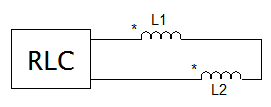
\includegraphics[scale=1]{schema1.png}
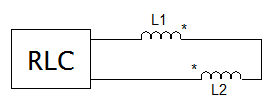
\includegraphics[scale=1]{schema2.png}
\caption{Sériové resp. antisériové schéma zapojení}
\end{figure}

\section{Postup měření}
Nejdříve si pomocí RLC měřiče změříme vlastní indukčnosti jednotlivých cívek. Poté změříme vzájemné indukčnosti s zapojením sériovém a antisériovém. Ze znalosti těchto hodnot můžeme spočítat celkovou vzájemnou indukčnost, činitel vazby a chybu měření.

\section{Naměřené a dopočítané hodnoty}
\captionof{table}{Naměřené a dopočítané hodnoty pro $f = 1kHz$}
\begin{tabular}{|c|c|c|c|c|}
\hline 
\multicolumn{2}{|c|}{Naměřené indukčnosti} & Rozsah RLC [mH] & \multicolumn{2}{|c|}{Absolutní chyby měření} \\ 
\hline 
$L_1[H]$ & 0,01619 & 100 & $\Delta L_1[H]$ & • \\ 
\hline 
$L_2[H]$ & 0,01073 & 100 & $\Delta L_2[H]$ & • \\ 
\hline 
$L_A[H]$ & 0,00930 & 10 & $\Delta L_A[H]$ & • \\ 
\hline
$L_B[H]$ & 0,04462 & 100 & $\Delta L_B[H]$ & • \\ 
\hline 
\end{tabular} \\\\\\
Vzájemná indukčnost:
\begin{equation}
M_x = \frac{L_A-L_B}{4} = \frac{0,00930-0,04462}{4} = -0,00883 H
\end{equation}
Činitel vazby:
\begin{equation}
\kappa = \frac{|M_x|}{\sqrt{L_1L_2}} = \frac{0,00883}{\sqrt{0,01619\cdot 0,01073}} = 0,67 [-]
\end{equation}

Chyby RLC měřiče jsou podle rozsahů:
\begin{itemize}
\item Rozsah 100mH = $\pm 0,3\% + (L_x/100000)\% + 5dgt$
\item Rozsah 10mH = $\pm 0,5\% + (L_x/100000)\% + 5dgt$
\end{itemize}
Kde $L_x$ jsou zobrazená čísla na dispeji, tzn. pokud $L=88,88H$, pak $L_x=8888$.
Absolutní chyba vzájemné indukčnosti je potom:
\begin{equation}
\Delta M_x = \Delta L_A - \Delta L_B = 0,000660 - 0,002818 = -0,002158H
\end{equation}
S tím, že:
$$\Delta L_1 = \pm 0,03\cdot 0,01619 + 0,01619\% + 0,00005 = \pm 0,000538 H$$
$$\Delta L_2 = \pm 0,03\cdot 0,01073 + 0,01073\% + 0,00005 = \pm 0,000373 H$$
$$\Delta L_A = \pm 0,05\cdot 0,00930 + 0,00930\% + 0,00005 = \pm 0,000330 H$$
$$\Delta L_B = \pm 0,03\cdot 0,04462 + 0,04462\% + 0,00005 = \pm 0,001409 H$$
Relativní chyba vzájemné indukčnosti:
\begin{equation}
\delta M_x = \frac{\Delta M_x}{M_x} = \frac{-0,002158}{-0,00883} = 0,244394 [-]
\end{equation}
Relativní chyba vlastní indukčnosti $L_1$:
\begin{equation}
\delta L_1 = \frac{\Delta L_1}{L_1} = \frac{0,000538}{0,01619} = 0,03323 [-]
\end{equation}
Relativní chyba vlastní indukčnosti $L_2$:
\begin{equation}
\delta L_2 = \frac{\Delta L_2}{L_2} = \frac{0,000373}{0,01073} = 0,034762 [-]
\end{equation}
Relativní chyba činitele vazby $\kappa$:
\begin{equation}
\delta \kappa = \delta M_x + \frac{\delta L_1}{2} + \frac{\delta L_2}{2} = 0,244394 + \frac{0,03323}{2} + \frac{0,034762}{2} = 0,27839 [-]
\end{equation}
Absolutní chyba činitele vazby $\kappa$:
\begin{equation}
\Delta \kappa = \delta \kappa \cdot \kappa = 0,27839 \cdot 0,67 = 0,186521 [-]
\end{equation}

\section{Závěr}
Číselné vyjádření vzájemného ovlivňování induktorů určuje činitel vazby. Ten by měl být v rozsahu $0-1$, což určuje zda se induktory vůcen neovlivňují (0), nebo jestli je mezi induktory těsná vazba (ideálně 1). V tomto případě vyšel činitel vazby $\kappa = 0,67$.

\section{Přístroje}
\begin{itemize}
\item RLC Meter Escort ELC 3131D, evid. 109599
\end{itemize}

\end{document}
